\section{Implementation}
\label{sec:implementation}

\begin{itemize}
  \item Extension of the library RxLua
  \item Why reactive?
    \url{http://www.reactivemanifesto.org/}
  \item ØMQ Lua bindings
  \item ØMQ queues with push/pull protocol - Fire-and-forget messaging: a messsaging pattern in which we do not expect a direct response to the message, as opposed to request-response protocols
\end{itemize}




\begin{figure}[t!]
  \centering
  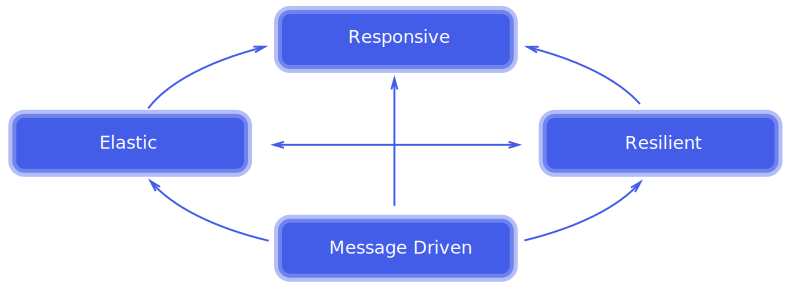
\includegraphics[width=.99\linewidth]{images/reactive-traits}
  \caption{Reactive traits.}
  \label{fig:reactive-traits}
\end{figure}


\begin{minipage}{\linewidth}
\begin{lstlisting}[language=LUA,caption={Process pipeline example, using the library RxLua},label=pipeline-example]
Rx.Observable.fromTable(people)
 :map(
   function(person)
     return person.age
   end
 )
 :filter(
   function(age)
     return age > 18
   end
 )
 :reduce(
   function(accumulator, age)
     accumulator[count] = (accumulator.count
       or 0) + 1
     accumulator[sum] = (accumulator.sum
       or 0) + age
     return accumulator
   end, {}
 )
 :subscribe(
   function(datas)
     print("Adult people average:",
       datas.sum / datas.count)
   end,
   function(err)
     print(err)
   end,
   function()
     print("Process complete!")
   end
 )
\end{lstlisting}
\end{minipage}
